\section{The U.S. airline industry after deregulation}\label{sec:09-industry}

The three studies at the center of this chapter use data on the U.S. airline industry between 1984 and 1987.
That period followed the end of federal economic regulation of the industry. This section describes the
institutions that a reader needs in order to interpret their regressions. We first explain how regulation
worked and why economists argued for its removal. We then describe the changes that followed deregulation,
the way the data define markets and products, and the devices that give a carrier an advantage at airports
where it is large.

\subsection{Regulation and the case for deregulation}\label{sec:09-regulation}

Until 1978 a federal agency, the \emph{Civil Aeronautics Board} (CAB), regulated interstate passenger air
travel in the United States. The agency decided which carriers could serve which routes, whether a carrier
could leave a route, and which fares it could charge. \citet[p.~1, n.~1]{BerryCarnallSpiller2006} summarize
the change in one sentence. Deregulation ``removed
restrictions on entry and exit and gave carriers the freedom to set fares.'' A carrier that wished to
serve a new interstate route needed the agency's approval.

When the price is fixed above cost and entry is closed, rivalry moves to the dimensions that the regulator
does not control. Flight frequency is the most important of them. A traveler values a schedule with many
departures because it shortens the wait between the time she wants to leave and the next flight. Economists
call this waiting cost \emph{frequency delay}, a concept that \citet{DouglasMiller1974} defined and
investigated \citep[p.~350]{Borenstein1989}. Suppose every carrier on a route must charge the regulated fare
$\bar p$, and a flight with $S$ seats costs $c_F$ to operate. At load factor $\mathit{LF}$, the share of
seats filled, the cost per passenger is
\begin{equation}\label{eq:09-cost-per-pax}
  \frac{c_F}{\mathit{LF}\cdot S}.
\end{equation}
An extra flight attracts some new travelers and takes others from rival carriers. The carrier that adds the
flight counts all the passengers it gains at the fare $\bar p$ and ignores the rivals' losses. Each carrier
therefore adds flights beyond the number that maximizes the carriers' joint profit, and load factors fall.
The margin between $\bar p$ and \eqref{eq:09-cost-per-pax} shrinks as flights are added. Travelers recover
part of it as shorter frequency delay, and the rest is spent on flying partly empty planes. The same
business-stealing logic produces excess entry in the model of \citet{MankiwWhinston1986}
(\cref{sec:02-entry}).

Two empirical studies made the case that regulation raised fares. \citet{Levine1965} compared fares on
intrastate routes in California, which the CAB did not regulate, with fares on regulated interstate routes.
The unregulated intrastate fares were much lower. \citet{Keeler1972} estimated the costs of efficient
carriers and found regulated fares far above them. Both studies shaped the policy debate, and
\cref{sec:01-early-studies} places them in the history of empirical industrial organization.

Economists also argued that deregulated airline markets would discipline themselves even when only one or two
carriers served a route. An aircraft can fly a different route tomorrow at little cost, so most of an
airline's capital is mobile across city pairs. Aircraft are often called ``capital on wings'' for this
reason. If a carrier can enter a route, undercut the incumbent and leave without loss, the threat of entry
alone keeps fares close to cost. This is the theory of contestable markets of \citet{BaumolPanzarWillig1982},
which \cref{sec:09-contest} develops. Congress passed the Airline Deregulation Act in 1978
\citep[p.~445]{WhinstonCollins1992}.

\subsection{Deregulation, entry, and the rise of hubs}\label{sec:09-hubs}

\citet[p.~445]{WhinstonCollins1992} summarize the first decade of deregulation. The Act, they write, ``led to
the entry of a large number of new carriers'' and to ``a dramatic change in existing carriers' route and fare
structures.'' It also brought ``a notable increase in the use of air transportation services.'' Three
developments matter for this chapter.
They are low-fare entry, the reorganization of networks around hubs, and a wave of mergers.

The emblematic new entrant was \emph{People Express}, a low-fare carrier that operated mainly out of Newark
airport in the New York area. Industry observers saw it as the embodiment of the innovations that
deregulation made possible \citep[pp.~446--447]{WhinstonCollins1992}. On the demand side, it introduced
``low-frill'' air travel. On the cost side, it used new operating procedures and paid lower labor costs than
the formerly regulated carriers (their n.~3). \citeauthor{WhinstonCollins1992} add two caveats. Incumbents
could perhaps have copied the procedures, and part of the labor-cost gap may reflect the quality or experience
of the work force. In 1984 and 1985 People Express entered 24 new domestic nonstop markets in which takeoff
and landing rights were not rationed, and 22 of them involved Newark (pp.~446, 450). \Cref{sec:09-wc} uses
these entry events to test the theory of \cref{sec:09-contest}.

The largest change in the established carriers' operations was the move from point-to-point networks to
hub-and-spoke networks. \citet[p.~1]{BerryCarnallSpiller2006} call it ``the almost complete shift in network
organization.'' In a \emph{point-to-point} network a carrier flies passengers nonstop between the cities they
wish to travel between. In a \emph{hub-and-spoke} network a carrier routes most passengers through one or a
few \emph{hub} airports, where they change planes. A \emph{segment}, or \emph{leg}, is a nonstop flight
between two airports, and a \emph{spoke} is a segment between a hub and another city. A passenger whose trip
starts and ends at the two endpoints of a segment is a \emph{local}, or \emph{origin and destination} (O\&D),
passenger of that city pair. A passenger who changes planes at the hub is a \emph{connecting} passenger there.
A \emph{through} passenger stays on board while the plane stops at an intermediate airport. Only local
passengers count as passengers of the city-pair market defined by a segment's endpoints
\citep[p.~349, n.~21]{Borenstein1989}.

A short count shows why hubs economize on segments. Consider $n$ outer cities and one hub city, $n+1$ cities
in all. The number of city pairs is
\begin{equation}\label{eq:09-citypairs}
  \binom{n+1}{2} = \frac{(n+1)n}{2}.
\end{equation}
Nonstop service in every pair needs one segment per pair, so it needs $\frac{(n+1)n}{2}$ segments. A
hub-and-spoke network needs only the $n$ spokes. It serves the $n$ hub markets nonstop and the remaining
\begin{equation*}
  \frac{(n+1)n}{2} - n = \frac{n(n-1)}{2}
\end{equation*}
city pairs with one change of plane at the hub. Each spoke carries its own hub market plus the $n-1$
connecting markets that start or end at its outer city. Traffic from $n$ city pairs therefore shares every
spoke. \Cref{fig:09-network} draws the case $n=4$. With $n=30$ outer cities, 30 spokes serve 465 city pairs.
This concentration of traffic on few segments lowers costs when the cost per passenger falls with the traffic
on a segment (\cref{ex:09-hubcost}). The price of the concentration is a longer trip with a connection for
most passengers.

\begin{figure}[htbp]
\centering
\begin{tikzpicture}[
  city/.style={circle, draw, thick, fill=white, minimum size=7mm, inner sep=0pt, font=\small},
  hub/.style={circle, draw, very thick, fill=gray!20, minimum size=8mm, inner sep=0pt, font=\small},
  leg/.style={thick, gray!60!black}]
  \begin{scope}
    \node[city] (H) at (90:1.6)  {$H$};
    \node[city] (A) at (162:1.6) {$A$};
    \node[city] (D) at (234:1.6) {$D$};
    \node[city] (C) at (306:1.6) {$C$};
    \node[city] (B) at (18:1.6)  {$B$};
    \foreach \u/\v in {H/A,H/B,H/C,H/D,A/B,A/C,A/D,B/C,B/D,C/D} \draw[leg] (\u) -- (\v);
    \node[font=\small, align=center] at (0,-2.45) {Point to point\\10 segments, 10 city pairs};
  \end{scope}
  \begin{scope}[xshift=6.6cm]
    \node[hub]  (H) at (0,0)        {$H$};
    \node[city] (A) at (-1.8,1.15)  {$A$};
    \node[city] (B) at (1.8,1.15)   {$B$};
    \node[city] (C) at (1.8,-1.15)  {$C$};
    \node[city] (D) at (-1.8,-1.15) {$D$};
    \draw[leg] (H) -- node[below, font=\footnotesize, pos=0.55] {$\ell_A$} (A);
    \draw[leg] (H) -- node[below, font=\footnotesize, pos=0.55] {$\ell_B$} (B);
    \draw[leg] (H) -- node[above, font=\footnotesize, pos=0.55] {$\ell_C$} (C);
    \draw[leg] (H) -- node[above, font=\footnotesize, pos=0.55] {$\ell_D$} (D);
    \draw[very thick, blue!60!black, shorten <=2pt]
      (A.east) to[bend left=14] (H.north west);
    \draw[-{Stealth[length=2.6mm]}, very thick, blue!60!black, shorten >=2pt]
      (H.north east) to[bend left=14] (B.west);
    \node[font=\footnotesize, blue!60!black, align=center] at (0,1.55) {itinerary $A \to H \to B$};
    \node[font=\small, align=center] at (0,-2.45) {Hub and spoke\\4 spokes, 10 city pairs};
  \end{scope}
\end{tikzpicture}
\caption{Point-to-point and hub-and-spoke networks on the same five cities. Nonstop service in every city
pair needs a segment for each of the $\binom{5}{2}=10$ pairs. A hub $H$ serves all $\frac{(n+1)n}{2} = 10$
pairs with $n=4$ spokes $\ell_A,\dots,\ell_D$. The four hub markets are served nonstop and the six other pairs
with one connection, such as the itinerary $A \to H \to B$, which uses spokes $\ell_A$ and $\ell_B$. Each spoke
carries the traffic of $n = 4$ city pairs.}
\label{fig:09-network}
\end{figure}

Observers disagree about what hubs do. One view holds that hub-and-spoke networks raise entry barriers and
drive up fares for passengers whose trips begin at a hub \citep{Borenstein1989,Borenstein1991}. Critics also
point to the extra connections and to congestion at hubs, where planes land and depart in
bunches \citep[p.~1, n.~2]{BerryCarnallSpiller2006}. A second view, held also by some airline executives, is
that hubs reduce costs \citep{CavesChristensenTretheway1984,BruecknerDyerSpiller1992,BruecknerSpiller1994}.
The success of carriers without hubs challenges the cost view. \citet[p.~1, n.~4]{BerryCarnallSpiller2006}
note that Southwest Airlines, which flies point to point, had been the only consistently profitable carrier
since deregulation. The two views are not mutually exclusive, as \citet{Berry1990} stressed. Hubs may raise
markups over marginal cost and lower marginal cost at the same time. Separating the two effects is the aim of
\citet{BerryCarnallSpiller2006}, whom we study in \cref{sec:09-bcs}.

Deregulation moved concentration in opposite directions at two levels of aggregation. Concentration within
city-pair markets fell, and concentration at airports rose
\citep[pp.~3, 27]{BerryCarnallSpiller2006}, who cite \citet{BruecknerSpiller1994} for the airport facts.
\citeauthor{BerryCarnallSpiller2006} suggest, without testing it, that hubs may explain both trends. Hubs
give price and cost advantages that ease a carrier's entry into new city pairs out of the hub. A dominant hub
carrier also draws business travelers away from its rivals at the hub, which leads them to cut service there
(p.~27). A carrier can therefore face more rivals on its average route while it controls most of the
departures at its hubs. \Cref{sec:09-dominance-sources} explains why dominance of an airport may raise fares
even where route concentration does not.

In 1986 and 1987 a wave of mergers consolidated the industry. Carriers with modest national market shares
proposed mergers that ``led to substantial regional and route-specific increases in concentration''
\citep[p.~446]{WhinstonCollins1992}. The Department of Transportation reviewed the mergers of
Texas Air and Eastern (1986), TWA and Ozark (1986), and USAir and Piedmont (1987)
\citep[p.~347, n.~14]{Borenstein1989}. The debates in these cases raised the questions of this chapter. Does
the structure of a single route matter when each carrier operates a national network? Can the threat of entry
discipline a carrier that dominates a route? \citet[p.~450]{WhinstonCollins1992} chose to study 1984 and 1985
partly because those years precede the merger wave.

\subsection{Markets, products, and data}\label{sec:09-data}

Empirical work on airlines defines a market as a directional trip from an origin to a destination. We index
such markets by $t$, as elsewhere in the book, and call the origin and the destination the two
\emph{endpoints} $e \in \{1,2\}$ of the market. \citet[p.~362]{Borenstein1989} and \citet{WhinstonCollins1992}
take the endpoints to be airports, so a market is an \emph{airport pair}. \citet[p.~7]{BerryCarnallSpiller2006}
take them to be cities, so that New York's three airports (Newark, La Guardia and Kennedy) form one origin.
In both cases direction matters. New York to Los Angeles is a different market from Los Angeles to New York.
Directional markets let characteristics of the origin, such as whether it is the carrier's hub, shift demand.
The choice between airport pairs and city pairs is substantive. It depends on whether flights from different
airports in one city compete, a question we return to in \cref{sec:09-dominance-sources}.

Within a market, carriers sell many products. \citet[p.~7]{BerryCarnallSpiller2006} define a \emph{product}
$j$ as a unique combination of carrier, itinerary and fare. Three products in the New York to Los Angeles
market might be a direct United flight at \$399, a direct United flight at \$299, and a United flight through
Chicago at \$299. Products with the same carrier and itinerary coexist at different fares because the tickets
carry different restrictions. Typical restrictions are advance-purchase requirements, Saturday-night stay
requirements and limits on the number of seats sold at a fare. The ticket data do not record them. This is one
reason the demand models of \cref{sec:09-pricing} include an unobserved product characteristic $\xi_{jt}$. We
write $\mathcal{J}_t$ for the set of products in market $t$, $f$ for carriers, and $q_{jt}$ for the number of
passengers who buy product $j$ in market $t$.

Itineraries differ in how they reach the destination. A \emph{nonstop} itinerary uses one segment with no
intermediate stop. A \emph{direct} itinerary uses one plane but may stop on the way. A \emph{connecting}
itinerary requires a change of plane. Let $\ell$ index carrier segments, that is, nonstop flights between two
airports operated by one carrier, and let $\mathcal{L}(j)$ be the set of segments in the itinerary of product
$j$. The \emph{density} of segment $\ell$ is the number of passengers on all itineraries that use it:
\begin{equation}\label{eq:09-density}
  Q_\ell = \sum_{t} \; \sum_{j \in \mathcal{J}_t :\, \ell \in \mathcal{L}(j)} q_{jt}.
\end{equation}
The outer sum runs over all markets. United's New York to Chicago spoke, for example, carries passengers to
many destinations beyond Chicago \citep[p.~8]{BerryCarnallSpiller2006}. Density links markets. A change in
the demand for one product changes the density, and possibly the cost, of every segment the product uses.

The data report several operating measures. An \emph{enplanement} is one passenger boarding a plane at an
airport, so enplanements count connecting passengers at every airport where they board. An
\emph{origination} is a passenger who begins a trip at the airport. A \emph{seat-mile} is one seat flown one
mile. A carrier's \emph{available seat-miles} on a segment, $\mathit{ASM}_\ell$, are the seats it offers times
the segment's distance, summed over flights. Its \emph{revenue passenger-miles}, $\mathit{RPM}_\ell$, are the
passengers it carries times the distance. The \emph{load factor} of the segment is the share of seats filled,
\begin{equation}\label{eq:09-loadfactor}
  \mathit{LF}_\ell = \frac{\mathit{RPM}_\ell}{\mathit{ASM}_\ell}.
\end{equation}
Let $d_t$ be the nonstop distance between the endpoints of market $t$. The \emph{yield} of product $j$ is its
fare per mile, $\frac{p_{jt}}{d_t}$. The \emph{circuity} of an itinerary is its total routing mileage divided
by $d_t$, so a nonstop trip has circuity one. \emph{Frequency} is the number of flights per period on a
segment. A \emph{slot} is the right to take off or land at an airport during a given time period. A
\emph{gate} is a physical facility, the building space and jetway through which passengers board
\citep[p.~347]{Borenstein1989}.

The empirical papers combine five sources.
\begin{itemize}
  \item The \emph{Origin and Destination Survey Databank 1A} (DB1A) of the U.S. Department of Transportation
  (DOT) is a random 10\% sample of tickets, compiled quarterly. Each record gives the carrier, the itinerary
  and its direction, the dollar fare and the distance \citep[p.~362]{Borenstein1989}. It also gives the number
  of sampled passengers who paid that fare in the quarter \citep[p.~19]{BerryCarnallSpiller2006}. It is
  the source of fares and of passenger counts by market.
  \item The \emph{Service Segment Data} are a census of the flights operated by the largest carriers of the
  regulated era. They count the passengers on board each flight, so they measure segment traffic more
  accurately than the 10\% ticket sample \citep[p.~363]{Borenstein1989}. \citet[p.~19]{BerryCarnallSpiller2006}
  use the Service Segment Databank DB27R, which reports each carrier's total monthly traffic on every nonstop
  segment it serves. These data give densities, load factors, aircraft sizes and frequencies.
  \item The \emph{Nonstop Market Data} are a similar census that covers all carriers.
  \citet[p.~363]{Borenstein1989} takes each carrier's enplanements at each airport from them.
  \item The \emph{Official Airline Guide}, published every two weeks, lists every scheduled flight between two
  airports with its carrier and aircraft type. \citet[p.~450]{WhinstonCollins1992} convert its flight counts
  into the seats each incumbent offered when an entry announcement was made.
  \item Daily stock returns from the \emph{Center for Research in Security Prices} (CRSP) supply the
  financial data for the event study of \cref{sec:09-wc} \citep[p.~451]{WhinstonCollins1992}.
\end{itemize}

Turning ticket records into market data requires conventions. \citet[p.~362]{Borenstein1989} splits each
round-trip ticket into two directional trips and assigns each trip half of the round-trip fare. A one-way
ticket is a single directional trip. The data vendor had already removed \emph{open-jaw trips}, whose return
starts or ends at a different city from the outbound trip, and \emph{circle trips}, which visit several cities
before returning. It had also removed tickets with more than one change of plane in either direction. Borenstein further drops tickets with a
first-class segment and tickets that use more than one carrier on a directional trip, called
\emph{interline} tickets. He also drops tickets that touch an airport outside the 200 largest U.S. airports,
and fares below \$10, which he presumes to be keypunch errors or frequent-flyer award trips.
\citet[p.~19]{BerryCarnallSpiller2006} keep only round-trip itineraries. They drop itineraries chosen by a
single sampled passenger and very low and very high fares, all as likely coding errors.

Fares vary widely within a market, even for one carrier and one itinerary. In about half of the markets with
more than one product, \citet[p.~19]{BerryCarnallSpiller2006} find that fares lie within 20\% of the market's
mean fare. In 10\% of these markets fares vary by more than 50\% from the mean. Because of this dispersion,
\citet{Borenstein1989} studies three points of each carrier's fare distribution on a route: the 20th, 50th
and 80th percentiles of the passenger-weighted distribution. He prefers the median to the mean because it is
less sensitive to reporting errors (p.~348, n.~19). In his sample the mean 80th-percentile fare is \$187,
against \$100 for the 20th percentile (his Table 4).

\citet[pp.~10--11, n.~10]{BerryCarnallSpiller2006} report a fat upper tail in the distribution of fares per
mile across tickets. Such a tail is inconsistent with a normal distribution. They suggest that the
distribution may be a bimodal mixture and fit a mixture of two normal distributions to it. The fitted
mixture puts weight 0.5987 on a component with mean 0.2375 and weight 0.4013 on a component with mean 0.5946.
The means are in dollars per mile, the unit of the fare-per-mile row of their Table~6. The footnote writes the
fit as $0.5987\,N(0.2375, 0.0781) + (1-0.5987)\,N(0.5946, 0.2752)$. It does not say whether the second argument of
$N$ is a standard deviation or a variance. Read as standard deviations, the fitted density has a shallow second
mode near 0.59. Read as variances, it has a single mode. The mixture's adjusted $R^2$ is 0.999, against 0.972
for a single normal distribution. A population with two groups of
travelers, one sensitive to price and one much less so, would generate this pattern. \Cref{sec:09-pricing}
builds the idea into a demand model with two consumer types.

\subsection{Sources of airport dominance}\label{sec:09-dominance-sources}

A carrier that handles most of the passengers at an airport may enjoy an advantage on every route that touches
the airport. Airline managers have said so openly, and they value dominance for the insulation from
competition it may give \citep[p.~345]{Borenstein1989}. The advantage can work in two ways. It can deter entry
into the dominant carrier's routes, and it can weaken the rivals that do enter. A device that does the second
also tends to do the first. \citet[p.~345]{Borenstein1989} separates advantages that arise naturally from
those that airline institutions create. The main natural advantage is reputation. A carrier that offers most
of the flights from a city becomes the carrier that local travelers know best. The institutional advantages
are frequent-flyer programs, bonus programs for travel agents, computer reservation systems, and control of
airport facilities. For each device we describe the mechanism and explain why it favors the carrier with the
most flights at an airport.

A \emph{frequent-flyer program} (FFP) gives a traveler a gift, usually free travel, after she has flown a given
amount on the carrier. Carriers first offered such programs in 1980 \citep[p.~346]{Borenstein1989}. Two
features make FFPs effective tools of loyalty. The reward schedule is nonlinear, since the marginal bonus rises
with the miles already accumulated. And the traveler often does not pay for her ticket, since her employer does.
The first feature ties a traveler to a single program.

\begin{lemma}[Nonlinear rewards concentrate purchases]\label{lem:09-ffp}
Let $R:[0,\infty) \to \R$ be convex with $R(0) = 0$. Then $R(x) + R(y) \le R(x+y)$ for all $x, y \ge 0$. A
traveler who flies $M$ miles and divides them between two programs with the same reward schedule $R$ therefore
earns the largest total reward by putting all $M$ miles in one program.
\end{lemma}

\begin{proof}
If $x + y = 0$ there is nothing to prove. Otherwise let $w = \frac{x}{x+y} \in [0,1]$. Convexity and
$R(0) = 0$ give
\begin{equation*}
  R(x) = R\big(w\,(x+y) + (1-w)\cdot 0\big) \le w\,R(x+y) + (1-w)\,R(0) = w\,R(x+y).
\end{equation*}
In the same way, $R(y) \le (1-w)\,R(x+y)$. Adding the two inequalities gives $R(x) + R(y) \le R(x+y)$. For
the second claim, take any split $x = m$ and $y = M - m$ with $m \in [0, M]$.
\end{proof}

Which program does the traveler choose? She picks the carrier she expects to fly most in the future
\citep[p.~346]{Borenstein1989}. That carrier has the most service on her routes and the most routes from her
home airport. The award also matters. The most common bonus is a free trip to a destination
of the traveler's choice, which is worth more when the carrier serves more destinations with more direct
service from her home. Both forces favor the carrier with the largest presence at the traveler's home airport.
Small carriers can form affiliated programs, but the costs of transacting, bargaining and coordinating such
arrangements are substantial. In their 1987 merger case, USAir and Piedmont argued that their small networks
made their programs less attractive than those of larger carriers (p.~346).

The second feature turns FFPs into what observers call kickbacks to business travelers
\citep[p.~346]{Borenstein1989}. The employee chooses the carrier and collects the bonus, while the employer pays
the fare. Write the employee's payoff from flying carrier $f$ as $v_f + b_f - \varsigma\, p_f$. Here $v_f$ is the
value of the flight, $b_f$ is the value of the bonus it earns, and $\varsigma \in [0,1]$ is the share of the fare
she bears herself. A business traveler has $\varsigma$ near zero. Her choice then responds weakly to fares and
strongly to bonuses, which raises the effectiveness of the program. The bonus is also untaxed compensation.
Borenstein notes that one can imagine an allocation of costs and benefits in which the only net loser is the
government (p.~346 and n.~9). Large buyers of travel, such as IBM and General Motors, had not objected strongly
to the programs. Low price sensitivity among business travelers is the ingredient that the two-type demand
model of \cref{sec:09-pricing} formalizes.

A \emph{travel agent commission override program} (TACO) pays a travel agent a bonus once the agent generates a
given volume of revenue for the carrier \citep[pp.~346--347]{Borenstein1989}. The bonus usually rises more
than proportionally with revenue, so \cref{lem:09-ffp} applies to the agent. Bonuses take the form of higher
commissions or of free travel that the agent can sell. A TACO works because the traveler cannot fully monitor
the agent or judge the quality of the agent's advice. In a 1988 survey of travel agents, 24\% said that such
programs ``usually'' influence their choice of airline for a customer, and 27\% said ``sometimes'' (p.~347).
Another 13\% answered ``rarely'' and 35\% ``never.'' As with FFPs, the carrier with the most flights from a
city offers the most chances to earn bonuses and the most valued bonuses.

\emph{Computer reservation systems} (CRSs) are the databases through which nearly all travel agents obtain
schedules and fares. Several carriers owned one. Despite federal rules on displays, many observers thought that
the owners biased the displays toward their own flights \citep[p.~347]{Borenstein1989}. Local dominance
reinforces the bias. In a city dominated by a carrier that owns a CRS, more agents choose that carrier's
system. They do so because it carries more timely information about the dominant carrier's flights, and
because their customers prefer that carrier for FFP and TACO reasons. The display bias then operates even for
travelers who do not prefer the dominant carrier. A DOT study found a strong correlation between a system's
share in a city and its owner's share of local traffic (p.~347, n.~13).

Serving an airport requires gates, and at some airports slots. A carrier that controls most of the gates can
refuse to sell or lease them to entrants. It may also influence the airport operator, usually a local
government, when the operator decides whether to expand the airport to accommodate entrants
\citep[p.~347]{Borenstein1989}. Where slots can be traded, a carrier that holds a dominant share of them can
also inhibit profitable entry (p.~348). In the period we study, four airports allocated slots under federal
rules (p.~351, n.~28, and \citealp[p.~450, n.~9]{WhinstonCollins1992}). They were Chicago O'Hare, New York's
Kennedy and La Guardia, and Washington National. Other congested airports operated under ``flow control,''
which Borenstein describes as essentially allocation by queuing.

Scarce airport capacity creates a measurement problem. When gates or runways are scarce, fares at an airport
can be high even if every carrier prices competitively. Such a premium is a \emph{scarcity rent}, the
competitive return to a scarce input. Borenstein insists that it must not be confused with market power
(p.~348), and he proposes a way to tell the two apart. If the scarce input is allocated competitively, its
shadow value is the same whichever carrier uses it. A carrier that uses a slot gives up the price at which it
could sell or lease it. The scarcity rent therefore raises every carrier's fares at the airport by the same
amount. Market power from dominance instead varies with each carrier's share of the airport's traffic. A
pricing equation of the form
\begin{equation}\label{eq:09-scarcity}
  \ln p_{ft} = \ln mc_{ft} + \varrho_k + \phi_1\, o_{fk} + (\text{other terms})
\end{equation}
separates the two. Here $p_{ft}$ is carrier $f$'s fare in market $t$ and $k$ is an endpoint airport of $t$.
The term $\varrho_k$ is a premium common to all carriers at $k$, and $o_{fk}$ is carrier $f$'s share of the
passengers who originate at $k$. The airport effect $\varrho_k$ is identified from the level of fares at $k$ relative to
other airports. The coefficient $\phi_1$ is identified from differences in shares among carriers that serve the
same airport. Borenstein adds a subtle point (p.~351, n.~27). Even the rents earned on inframarginal uses of a
scarce input raise prices by the same amount in every use, if all uses are competitive. Rents then differ
across uses only because production costs differ. \Cref{sec:09-borenstein} implements this idea with airport
terms restricted to be equal across carriers.

The last question concerns the boundaries of markets. Do flights from Kennedy airport to Detroit discipline
fares on flights from La Guardia to Detroit? Antitrust analyses usually answer with cross-elasticities of
demand. \citet[p.~348]{Borenstein1989} argues that this ignores demand segmentation. Travelers with low values
of time may switch readily between the two airports, while travelers with high values of time may not. If a
carrier can sort the two groups, competition for the first group need not discipline the fares charged to the
second. Restricted discount fares sort travelers by their time values. Competing airports in a city should
therefore restrain discount fares more than the fares paid by business travelers. Borenstein treats flights
from different airports as separate markets. \Cref{sec:09-wc} tests whether incumbents at other airports in
the same city lose value when a low-fare carrier enters.

These mechanisms share a prediction. A carrier's presence at an endpoint airport, measured by its share of the
passengers who begin their trips there, should raise its fares on routes from that airport. The effect should
be strongest for fares paid by business travelers, who respond to FFPs and are least sensitive to price. The
empirical work cannot separate the individual devices \citep[p.~362]{Borenstein1989}. \citet{Borenstein1989}
measures dominance by route and airport shares (\cref{sec:09-borenstein}).
\citet{BerryCarnallSpiller2006} measure it by the size of the carrier's hub network at the origin
(\cref{sec:09-bcs}). \citet{CilibertoWilliams2010} later measure the role of gate control directly
(\cref{sec:09-synthesis}).

\section{Contestability, entry, and incumbent profits}\label{sec:09-contest}

The theory of contestable markets gave the strongest argument that deregulated airline markets would perform
well even when few carriers served them. It is also the benchmark that all three studies in this chapter
reject. This section states the theory, proves its main results and shows that an equilibrium may fail to
exist. It then explains why airlines seemed a natural application, why the theory is fragile, and what
testable predictions it makes. The last subsection
derives what an incumbent's loss of value at an entry announcement reveals, which is the logic of the event
study in \cref{sec:09-wc}.

\subsection{Contestable markets}\label{sec:09-contestable}

The theory is due to \citet{BaumolPanzarWillig1982} and \citet{Baumol1982}. We follow the single-product
exposition of \citet[sec.~8.1.2]{Tirole1988}, which states the first three definitions below in the same form.
Tirole defines a perfectly contestable market as one in which any equilibrium configuration must be
sustainable. This requirement is the last sentence of \cref{def:09-contestable}. Conditions (i) to (iii) of
that definition spell out the assumptions behind it. Tirole places (i) and (ii) in his setup and (iii) in his
account of hit-and-run entry. The definitions extend to several products by treating outputs and prices as vectors. Market demand $Q(p)$ is
continuous and strictly decreasing wherever it is positive. Every firm, active or potential, has the same cost
function $C(q)$, with $C(0) = 0$. The condition $C(0) = 0$ means that a firm that produces nothing
pays nothing, so no cost is sunk. A fixed cost is allowed, as in $C(q) = F + cq$ for $q > 0$, but it must be
avoidable by shutting down.

\begin{definition}[Industry configuration]\label{def:09-configuration}
An \emph{industry configuration} $(m; q_1, \dots, q_m; p)$ is a number of active firms $m \ge 1$, their outputs
$q_1, \dots, q_m > 0$, and a common price $p$. The other firms are \emph{potential entrants} and produce nothing.
\end{definition}

\begin{definition}[Feasible configuration]\label{def:09-feasible}
A configuration is \emph{feasible} if supply equals demand and no active firm loses money:
\begin{equation*}
  \sum_{i=1}^m q_i = Q(p) \qquad\text{and}\qquad p\,q_i - C(q_i) \ge 0 \quad\text{for } i = 1, \dots, m.
\end{equation*}
\end{definition}

\begin{definition}[Sustainable configuration]\label{def:09-sustainable}
A feasible configuration is \emph{sustainable} if no entry plan earns a positive profit at the incumbents'
price. That is, there is no pair $(p^e, q^e)$ with
\begin{equation*}
  p^e \le p, \qquad 0 < q^e \le Q(p^e), \qquad\text{and}\qquad p^e q^e - C(q^e) > 0.
\end{equation*}
\end{definition}

The entry plan reflects the timing the theory assumes. An entrant that matches or undercuts the incumbents'
price can sell any quantity up to the market demand at its own price. It evaluates its profit while
incumbents keep their price unchanged.

\begin{definition}[Perfectly contestable market]\label{def:09-contestable}
A market is \emph{perfectly contestable} if three conditions hold. (i) Entrants have the same cost function
$C$ as incumbents and face the same market demand. (ii) There are no sunk costs, so a firm that exits recovers
every cost it incurred on entry. (iii) Consumers switch at once to a lower price, while incumbents change
their prices only with a lag. An equilibrium of a perfectly contestable market is a sustainable configuration.
\end{definition}

Conditions (ii) and (iii) together make \emph{hit-and-run entry} possible. An entrant can come in, undercut
the incumbents, earn profits until they respond, and leave without loss. Sustainability is the requirement
that no such plan pays. Two results follow.

\begin{proposition}[Zero profit]\label{prop:09-contest-zero}
In a sustainable configuration, every active firm earns zero economic profit.
\end{proposition}

\begin{proof}
Feasibility gives $\pi_i \equiv p\,q_i - C(q_i) \ge 0$ for every active firm. Suppose that $\pi_i > 0$ for
some firm $i$. Consider the entry plan $(p^e, q^e) = (p - \epsilon, q_i)$ with $0 < \epsilon < \frac{\pi_i}{q_i}$.
It satisfies $p^e \le p$. Because demand is decreasing, $Q(p - \epsilon) \ge Q(p) \ge q_i$, so the plan
satisfies $q^e \le Q(p^e)$. Its profit is
\begin{equation*}
  (p - \epsilon)\,q_i - C(q_i) = \pi_i - \epsilon\, q_i > 0.
\end{equation*}
This contradicts sustainability. Hence $\pi_i = 0$.
\end{proof}

\begin{proposition}[Marginal-cost pricing with two or more firms]\label{prop:09-contest-mc}
Suppose $C$ is differentiable at each active firm's output. In a sustainable configuration with $m \ge 2$
active firms, $p = C'(q_i)$ for every active firm $i$.
\end{proposition}

\begin{proof}
By \cref{prop:09-contest-zero}, $p\,q_i = C(q_i)$ for every active firm.

Suppose first that $p > C'(q_i)$ for some $i$. Because another firm is active, $Q(p) = \sum_k q_k > q_i$.
Hence $q_i + h \le Q(p)$ for every small $h > 0$, and the plan $(p, q_i + h)$ is admissible. Its profit is
\begin{align*}
  p\,(q_i + h) - C(q_i + h)
  &= \big[p\,q_i - C(q_i)\big] + p\,h - \big[C(q_i + h) - C(q_i)\big] \\
  &= 0 + p\,h - C'(q_i)\,h + o(h) \\
  &= h\,\big(p - C'(q_i)\big) + o(h),
\end{align*}
which is positive for $h$ small enough. This contradicts sustainability.

Suppose next that $p < C'(q_i)$. For small $h \in (0, q_i)$ the plan $(p, q_i - h)$ is admissible, since
$q_i - h < Q(p)$. Its profit is
\begin{align*}
  p\,(q_i - h) - C(q_i - h)
  &= \big[p\,q_i - C(q_i)\big] - p\,h + \big[C(q_i) - C(q_i - h)\big] \\
  &= 0 - p\,h + C'(q_i)\,h + o(h) \\
  &= h\,\big(C'(q_i) - p\big) + o(h),
\end{align*}
which is again positive for $h$ small enough. Hence $p = C'(q_i)$.
\end{proof}

The second step of the proof does not use $m \ge 2$, so even a single active firm must price at or above
marginal cost. The first step does use it. A lone incumbent sells the whole market demand at its price, so an
entrant cannot sell more at the same price.

\begin{corollary}[Efficient scale]\label{cor:09-contest-scale}
In a sustainable configuration with $m \ge 2$ firms, each active firm produces where average cost
$AC(q) = \frac{C(q)}{q}$ equals marginal cost. If $AC$ is U-shaped and its derivative vanishes only at its
minimum, each firm therefore produces at the bottom of its average cost curve and $p = \min_q AC(q)$.
\end{corollary}

\begin{proof}
\Cref{prop:09-contest-zero} gives $p = \frac{C(q_i)}{q_i} = AC(q_i)$, and \cref{prop:09-contest-mc} gives
$p = C'(q_i)$. Hence $AC(q_i) = C'(q_i)$. Differentiating average cost,
\begin{equation*}
  AC'(q) = \frac{C'(q)\,q - C(q)}{q^2} = \frac{C'(q) - AC(q)}{q},
\end{equation*}
so $AC'(q_i) = 0$. Under the stated shape, the only such point is the minimum of $AC$.
\end{proof}

With a single firm the zero-profit condition becomes $p\,Q(p) = C(Q(p))$, so price equals average cost at the
quantity demanded. The next proposition treats the natural monopoly case.

\begin{proposition}[Sustainable natural monopoly]\label{prop:09-contest-monopoly}
Suppose $AC(q)$ is strictly decreasing for $q > 0$. Let $P(q)$ be inverse demand, and suppose $P$ and $AC$ cross
exactly twice, at $q_L < q_H$, with $P(q) > AC(q)$ for $q \in (q_L, q_H)$ and $P(q) < AC(q)$ for
$q \notin [q_L, q_H]$. Let $p^c = P(q_H)$. Then the monopoly configuration $(1; q_H; p^c)$ is sustainable, and it
is the only sustainable configuration. Among prices at which a firm serving the whole market breaks even,
$p^c$ is the lowest, so it maximizes consumer and total surplus.
\end{proposition}

\begin{proof}
We first show that the configuration is sustainable. It is feasible because $p^c q_H = AC(q_H)\,q_H = C(q_H)$. Take any
entry plan with $p^e \le p^c$ and $0 < q^e \le Q(p^e)$. Because $p^e \le p^c$, $Q(p^e) \ge q_H$. Because $AC$ is
decreasing and $q^e \le Q(p^e)$, $AC(q^e) \ge AC(Q(p^e))$. The plan's profit is therefore
\begin{equation*}
  q^e\big(p^e - AC(q^e)\big) \le q^e\big(p^e - AC(Q(p^e))\big)
  = q^e\big(P(Q(p^e)) - AC(Q(p^e))\big) \le 0,
\end{equation*}
where the last inequality holds because demand lies on or below average cost at quantities of at least $q_H$.

We next show uniqueness. Consider any sustainable configuration, and suppose it has $m \ge 2$ firms. By
\cref{prop:09-contest-zero}, $p = AC(q_i)$ for each firm, and $q_i < Q(p)$. Because $AC$ is strictly decreasing,
$AC(Q(p)) < AC(q_i) = p$. The plan $(p, Q(p))$ then earns $Q(p)\big(p - AC(Q(p))\big) > 0$, a contradiction.
So $m = 1$ and $p = AC(Q(p))$, which means $p \in \{P(q_L), P(q_H)\}$. If $p = P(q_L)$, an entrant can choose
any $q^e \in (q_L, q_H)$ at the price $P(q^e) < P(q_L)$ and earn $q^e\big(P(q^e) - AC(q^e)\big) > 0$. Hence
$p = P(q_H) = p^c$.

Finally, a single firm serving the market breaks even exactly at the prices $P(q_L)$ and $P(q_H)$. Its
profit is zero at both, so total surplus equals consumer surplus, which is decreasing in price. The lower
price $p^c$ therefore gives the larger surplus.
\end{proof}

The price $p^c$ is the \emph{second-best} price. A planner who cannot subsidize the firm, and who must
therefore let it cover its costs, would choose it. Marginal-cost pricing would give more surplus. At the
quantity $q$ sold at that price, however, the firm would lose $C(q)-C'(q)\,q>0$, because marginal cost lies
below a falling average cost. The loss equals the fixed cost $F$ when $C(q)=F+cq$.

\begin{example}[A contestable natural monopoly]\label{ex:09-contest}
Let $C(q) = F + cq$ for $q > 0$ with $C(0) = 0$, so the fixed cost $F$ is avoidable. Then
$AC(q) = c + \frac{F}{q}$ falls with $q$ and marginal cost is $c$. Let demand be $Q(p) = 12 - p$, with $c = 2$
and $F = 8$. Setting $P(q) = AC(q)$ gives $12 - q = 2 + \frac{8}{q}$, or $q^2 - 10q + 8 = 0$. The roots are
$q_L = 5 - \sqrt{17} \approx 0.88$ and $q_H = 5 + \sqrt{17} \approx 9.12$. The sustainable price is
$p^c = 12 - q_H = 7 - \sqrt{17} \approx 2.88$. An unthreatened monopolist would set marginal revenue
$12 - 2q$ equal to $c = 2$. It would sell 5 units at $p^m = 7$ and earn $5 \times 5 - 8 = 17$. Under perfect
contestability, the same single firm charges $2.88$ and earns zero. \Cref{fig:09-contest} draws the example.

The same price solves the zero-profit condition in price form, $(p^c - c)\,Q(p^c) = F$
\citep[sec.~8.1.2]{Tirole1988}. Substituting the example's values,
\begin{align*}
  (p - 2)(12 - p) &= 8, \\
  p^2 - 14p + 32 &= 0, \\
  p &= 7 \pm \sqrt{17}.
\end{align*}
The larger root, $7 + \sqrt{17} \approx 11.12$, is the price $P(q_L)$ at the left crossing. The smaller root is
$p^c$. For any cost function $C(q) = F + cq$ with a viable monopoly, \citeauthor{Tirole1988} draws three
conclusions. (1) A single firm operates, so the fixed cost is not duplicated. (2) This firm earns zero profit.
(3) Price equals average cost, and the allocation is \emph{constrained efficient}. It is the best allocation
that a planner can reach without subsidizing the firm. The first-best price $c$ would make the firm lose $F$.
\end{example}

\begin{figure}[htbp]
\centering
\begin{tikzpicture}
\begin{axis}[
  width=0.78\textwidth, height=0.45\textwidth,
  axis lines=left,
  xmin=0, xmax=13, ymin=0, ymax=12.5,
  xlabel={Output $q$}, ylabel={Price and cost},
  xtick={5, 9.123}, xticklabels={$Q(p^m)$, $Q(p^c)$},
  ytick={2, 2.877, 7}, yticklabels={$c$, $p^c$, $p^m$},
  every axis x label/.style={at={(current axis.right of origin)}, anchor=north east, yshift=-14pt},
  every axis y label/.style={at={(current axis.above origin)}, anchor=south, yshift=2pt},
  tick label style={font=\footnotesize},
  clip=false]
  \addplot[name path=dem, thick, blue!70!black, domain=0:12, samples=2] {12-x};
  \addplot[name path=ac, thick, black, domain=0.8:12.6, samples=150] {2+8/x};
  \addplot[thick, red!70!black, domain=0:12.6, samples=2] {2};
  \addplot[thick, dashed, blue!70!black, domain=2.5:6, samples=2] {12-2*x};
  \addplot[gray!25] fill between[of=dem and ac, soft clip={domain=0.877:9.123}];
  \draw[dotted] (axis cs:5,0) -- (axis cs:5,7) -- (axis cs:0,7);
  \draw[dotted] (axis cs:9.123,0) -- (axis cs:9.123,2.877) -- (axis cs:0,2.877);
  \fill (axis cs:5,7) circle (2pt) node[above right] {$M$};
  \fill (axis cs:9.123,2.877) circle (2pt) node[above right] {$S$};
  \node[anchor=west, font=\small] (aclab) at (axis cs:6.6,10.9) {$AC(q) = c + \frac{F}{q}$};
  \draw[-{Stealth[length=2mm]}, thin] (aclab.west) -- (axis cs:1.32,8.06);
  \node[anchor=west, font=\small, blue!70!black] at (axis cs:11.2,1.3) {$P(q)$};
  \node[anchor=west, font=\small, blue!70!black] at (axis cs:5.95,0.9) {$MR(q)$};
  \node[anchor=west, font=\small, red!70!black] at (axis cs:12.6,2) {$MC = c$};
  \node[font=\footnotesize] at (axis cs:6.3,4.25) {$\pi > 0$};
\end{axis}
\end{tikzpicture}
\caption{A contestable natural monopoly. Average cost $AC(q) = c + \frac{F}{q}$ lies above marginal cost $c$
everywhere. An unthreatened monopolist would produce where marginal revenue $MR(q)$ equals $c$ and charge
$p^m$ (point $M$). In the shaded region inverse demand $P(q)$ lies above average cost, so any price in it
earns a positive profit $\pi = p\,Q(p) - C(Q(p))$ and invites hit-and-run entry. The only sustainable configuration is a single firm at
$S$, where demand cuts average cost from above and $p^c = AC(Q(p^c))$. The curves use $c = 2$, $F = 8$ and
$P(q) = 12 - q$, which give $p^m = 7$ and $p^c = 7 - \sqrt{17} \approx 2.88$.}
\label{fig:09-contest}
\end{figure}

Three features of the theory explain its appeal for policy, and a fourth limits it.

\begin{remark}[Structure does not determine performance]\label{rem:09-structure}
In a perfectly contestable market, the price is pinned down by cost and demand alone. A monopoly and an
industry of many firms can both price at average cost. Concentration therefore carries no information about
market power, and the structure-conduct-performance regressions of \cref{ch:intro} have no basis.
\end{remark}

\begin{remark}[Potential competition]\label{rem:09-potential}
Potential entrants discipline incumbents as well as actual rivals do. The incumbents need not face any active
rival. They price at average cost because a price above it would invite entry.
\end{remark}

\begin{remark}[Efficiency]\label{rem:09-efficiency}
Sustainable configurations are efficient in the second-best sense. With two or more firms, price equals
marginal cost and each firm produces at minimum average cost (\cref{cor:09-contest-scale}). With one firm,
price equals average cost at the lowest break-even price (\cref{prop:09-contest-monopoly}).
\end{remark}

\begin{remark}[Existence]\label{rem:09-existence}
A sustainable configuration need not exist. \citet[sec.~8.1.2]{Tirole1988} reports that
\citet{BaumolPanzarWillig1982} show that natural monopolies may fail to be sustainable for some demand and
cost functions. There may be no price and outputs at which firms break even, the market clears, and no entry
plan at a lower or equal price earns a profit. A constrained efficient market structure can then be upset by
entry. The next proposition works out the case of Tirole's Exercise 8.1.
\end{remark}

\begin{proposition}[No sustainable configuration]\label{prop:09-nonexist}
Let $AC$ be U-shaped. It falls strictly below an \emph{efficient scale} $q^*$ and rises strictly above it, with minimum $a^* = AC(q^*)$. Suppose that demand at the minimum
average cost exceeds the efficient scale but is not an integer multiple of it:
\begin{equation*}
  Q(a^*) > q^* \qquad\text{and}\qquad \frac{Q(a^*)}{q^*} \notin \{2, 3, \dots\}.
\end{equation*}
Then no configuration is sustainable. This covers the case in which demand cuts average cost slightly to
the right of the efficient scale, so that $q^* < Q(a^*) < 2q^*$.
\end{proposition}

\begin{proof}
Suppose a sustainable configuration $(m; q_1, \dots, q_m; p)$ exists, and let $P$ be inverse demand. The
argument covers every $m \ge 1$ and uses no derivative.

First, the price equals the minimum average cost. Feasibility gives $p \ge AC(q_i) \ge a^*$ for every active
firm. Because demand is decreasing and $Q(a^*) > q^*$, we also have $P(q^*) > a^*$. Suppose that $p > a^*$,
and consider the entry plan
\begin{equation*}
  p^e = \min\{p,\, P(q^*)\}, \qquad q^e = q^*.
\end{equation*}
It satisfies $p^e \le p$. Because $p^e \le P(q^*)$, demand at $p^e$ is at least $q^*$, so $q^e \le Q(p^e)$. Its
profit is
\begin{equation*}
  p^e q^* - C(q^*) = q^*\,(p^e - a^*) > 0,
\end{equation*}
since both $p$ and $P(q^*)$ exceed $a^*$. This contradicts sustainability. Hence $p = a^*$.

Second, every active firm produces at the efficient scale. With $p = a^*$, feasibility gives
$AC(q_i) \le a^*$. Since $a^*$ is the minimum of $AC$, $AC(q_i) = a^*$. The U shape makes $q^*$ the unique
minimizer, so $q_i = q^*$ for every $i$. Market clearing then gives $Q(a^*) = m\,q^*$.

Third, this equation contradicts the assumptions on demand. If $m = 1$, it reads $Q(a^*) = q^*$, which
contradicts $Q(a^*) > q^*$. If $m \ge 2$, it gives $\frac{Q(a^*)}{q^*} = m \in \{2, 3, \dots\}$, which
contradicts the integer condition. Hence no configuration is sustainable.
\end{proof}

The entrant in the proof matches or undercuts the incumbents' price but produces only at its efficient scale. It
leaves part of the demand unserved, which the definition of sustainability allows. A numerical case shows the
logic. Let $C(q) = 1 + q^2$ for $q > 0$, so $AC(q) = \frac{1}{q} + q$, with $q^* = 1$ and $a^* = 2$. Let
$Q(p) = 3.5 - p$, so $Q(a^*) = 1.5$. Two firms at the efficient scale would supply 2 units at the price 2,
more than the 1.5 units demanded. A single firm breaks even where $3.5 - q = \frac{1}{q} + q$, that is,
\begin{equation*}
  4q^2 - 7q + 2 = 0, \qquad q = \frac{7 \pm \sqrt{17}}{8}.
\end{equation*}
At the right crossing, $q \approx 1.39$ and the price is $\frac{21 - \sqrt{17}}{8} \approx 2.11$. An entrant that
charges the same price and produces one unit earns $\frac{5 - \sqrt{17}}{8} \approx 0.11 > 0$. \citet{BrockScheinkman1983} study a weaker test, \emph{quantity sustainability}, in which the entrant expects
the incumbent's output to stay fixed after entry \citep[sec.~8.1.2, n.~12]{Tirole1988}. The price then adjusts
to clear the market for the combined output. Brock and Scheinkman show that, under some assumptions, the
crossing allocation of a single-product industry passes this test. In the example, an entrant that produces
$q^e$ faces the price $2.11 - q^e$ and earns $q^e\,(2.11 - q^e) - 1 - (q^e)^2$. This profit is largest at
$q^e \approx 0.53$ and equals about $-0.44$ there. Every such plan therefore loses money.

\begin{remark}[Contestability as Bertrand competition]\label{rem:09-bertrand}
A two-stage game yields the contestable outcome \citep[sec.~8.1.2]{Tirole1988}. All firms first set prices
simultaneously. They then choose outputs, and a positive output means entry. This timing reverses that of
the capacity-then-price game of \citet{KrepsScheinkman1983} (\cref{rem:09-ks}). Take the setting of
\cref{prop:09-contest-monopoly}. Let every firm set $p^c$, let one firm supply $Q(p^c)$, and let the others
produce nothing. Every firm earns zero. A firm that sets $p < p^c$ and produces $q \in (0, Q(p)]$ earns
\begin{equation*}
  q\,\big(p - AC(q)\big) \le q\,\big(p - AC(Q(p))\big) < 0 .
\end{equation*}
The first inequality holds because $AC$ is decreasing and $q \le Q(p)$. The second holds because
$Q(p) > q_H$, where demand lies below average cost. A firm that sets a price above $p^c$ sells nothing, since
another firm supplies the whole demand at $p^c$. No deviation pays, so the profile is an equilibrium. Tirole
sketches why it is the only one (n.~9). As \citeauthor{BaumolPanzarWillig1982} note, perfect contestability
thus extends Bertrand competition to markets with increasing returns to scale. With constant marginal cost
and no fixed cost, the same game gives the Bertrand price $c$. The game also makes the theory's timing
explicit. Prices are fixed while firms choose quantities and entry. \Cref{sec:09-contest-fail} questions
this assumption.
\end{remark}

\subsection{Why airlines, and why the theory may fail}\label{sec:09-contest-fail}

Airlines looked like the textbook case of a contestable industry. Aircraft, the largest capital asset, can be
moved from one city pair to another at low cost. Entry into a new route between two airports a carrier already
serves needs little capital that is specific to the route. The ideal of hit-and-run entry thus seemed close to
reality. If it held, deregulated routes would be priced near average cost even when only one carrier served
them, and concentration on a route would not be a concern for policy. \citet{BaileyPanzar1981} made this
argument for city-pair markets, as \citet[sec.~8.1.2, n.~11]{Tirole1988} reports. Airline service has returns
to scale, but its fixed costs are not sunk. Aircraft can be redeployed at little cost, and municipalities bear
the sunk costs of runways, towers and ground facilities. Bailey and Panzar offered evidence that single-carrier
routes, almost 70\% of all routes, were priced roughly competitively on long hauls just after deregulation.
\citet{BaileyGrahamKaplan1985} and others found instead that fares rise with concentration. Tirole describes
that relation as statistically strong but not economically large.

The theory is fragile, however, in a way that matters for airlines. Its conclusions require exactly zero sunk
costs together with a lag before incumbents respond. Two observations of \citet[secs.~8.1.1--8.1.2]{Tirole1988}
frame the problem. First, fixed and sunk costs differ only in degree. A fixed cost does not vary
with output and is committed for a short time, which defines the length of a period. A sunk cost yields
benefits over a long horizon and can never be recovered. A machine rented by the month is a fixed cost, and a
machine that cannot be resold is sunk. What matters is how long a commitment lasts compared with the time it
takes to change prices. Second, the hit-and-run story assumes that prices adjust more slowly than entry
decisions. Critics argue the reverse. In railroads, entry requires buying parcels of land, often with powers
of eminent domain, and then engineering and building the line. Fares can change much sooner. Tirole adds
that price adjustment ``may be even faster in the airline industry, where opening a new route is a relatively
fast process.'' Suppose the incumbent cuts its price soon after entry, measured against the time the entrant
needs to invest. Hit-and-run entry then does not pay, because a natural monopoly leaves no room for two firms
that compete in prices.

A simple model makes the point precise. Suppose that entry requires a sunk investment
$K > 0$ and that incumbents can change fares within $T$ periods of entry. In this subsection only, $T$ denotes
this response lag, and $\delta \in (0,1)$ is a per-period discount factor. An entrant that undercuts a
monopolist earns a profit $\pi^e$ per period until the incumbent responds. After the response the entrant earns
$\pi^d \ge 0$ per period, for example $\pi^d = 0$ if the two firms then compete in prices with identical
costs. Entry pays if and only if
\begin{equation}\label{eq:09-hitrun}
  \sum_{\tau=0}^{T-1} \delta^{\tau}\,\pi^e + \sum_{\tau=T}^{\infty} \delta^{\tau}\,\pi^d \ge K .
\end{equation}
Summing the two geometric series gives the equivalent condition
\begin{equation}\label{eq:09-hitrun-closed}
  \pi^e\,\frac{1 - \delta^{T}}{1 - \delta} + \delta^{T}\,\frac{\pi^d}{1 - \delta} \ge K .
\end{equation}
The first term is the value of the hit-and-run window. It is at most $T\pi^e$, and $\pi^e$ cannot exceed the
monopoly profit per period. Because profit accrues per unit of time, the window's value shrinks to zero as the
response becomes faster.

\begin{proposition}[The fragility of contestability]\label{prop:09-fragility}
Suppose that after incumbents respond the entrant earns $\pi^d = 0$, and let $\pi^m$ be the monopoly profit per
period. (a) If $K = 0$, hit-and-run entry against an incumbent that earns a positive profit pays for every
response lag $T \ge 1$. (b) If $K > 0$, entry against the monopoly price is unprofitable whenever
$\pi^m\,\frac{1-\delta^T}{1-\delta} < K$. In particular, it is unprofitable whenever $T\pi^m < K$, so a fast
enough response protects the monopoly price for any $K > 0$.
\end{proposition}

\begin{proof}
With $\pi^d = 0$, condition \eqref{eq:09-hitrun-closed} reads $\pi^e\,\frac{1-\delta^T}{1-\delta} \ge K$.
(a) An incumbent profit $\pi_i > 0$ leaves room for an undercutting plan with $\pi^e > 0$, as in the proof
of \cref{prop:09-contest-zero}. With $K = 0$ and $T \ge 1$, the left side is at least $\pi^e > 0 = K$. (b) Any
entrant earns $\pi^e \le \pi^m$ per period, so the left side is at most $\pi^m\,\frac{1-\delta^T}{1-\delta}$.
Since $\delta^\tau \le 1$ for every $\tau$, this bound is itself at most $T\pi^m$.
\end{proof}

The proposition shows a discontinuity. At $K = 0$ the price equals average cost for every positive response
lag. With any positive sunk cost and a fast response, the incumbent can charge the monopoly price. Entry then
depends on the second term of \eqref{eq:09-hitrun-closed}, the profit an entrant expects to earn after
incumbents respond. The incumbent's current price no longer matters for the entry decision. \Cref{fig:09-hitrun}
illustrates the threshold.

\begin{figure}[htbp]
\centering
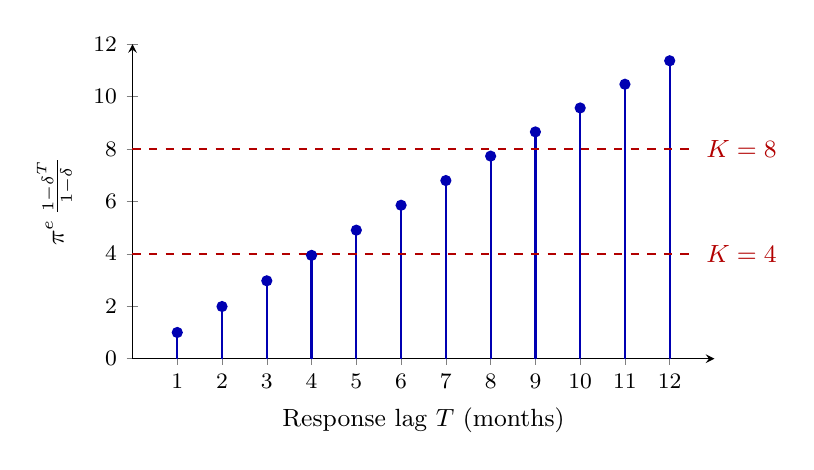
\begin{tikzpicture}
\begin{axis}[
  width=0.74\textwidth, height=0.46\textwidth,
  axis lines=left,
  xmin=0, xmax=13, ymin=0, ymax=12,
  xtick={1,2,...,12}, ytick={0,2,...,12},
  xlabel={Response lag $T$ (months)},
  ylabel={$\pi^e\,\frac{1-\delta^{T}}{1-\delta}$},
  tick label style={font=\footnotesize}, label style={font=\small},
  clip=false]
  \addplot[ycomb, thick, blue!70!black, mark=*, mark size=1.6pt, domain=1:12, samples=12]
    {(1-0.99^x)/(1-0.99)};
  \addplot[thick, dashed, red!70!black, domain=0:12.6, samples=2] {4};
  \addplot[thick, dashed, red!70!black, domain=0:12.6, samples=2] {8};
  \node[anchor=west, font=\small, red!70!black] at (axis cs:12.6,4) {$K = 4$};
  \node[anchor=west, font=\small, red!70!black] at (axis cs:12.6,8) {$K = 8$};
\end{axis}
\end{tikzpicture}
\caption{The value of hit-and-run entry when the entrant earns nothing after incumbents respond. Bars show the
discounted profit earned during a response lag of $T$ months, with $\pi^e = 1$ per month and a monthly discount
factor $\delta = 0.99$. Entry pays only if the bar reaches the sunk cost. With $K = 4$ it requires a lag of at
least 5 months, and with $K = 8$ at least 9 months. With $K = 0$ any lag makes entry profitable.}
\label{fig:09-hitrun}
\end{figure}

Airline markets have several sources of sunk costs. An entrant must set up gates, counters and other airport
facilities at a new station, and it must advertise to make itself known to local travelers. In his conclusion,
\citet[p.~362]{Borenstein1989} names advertising and the setup of airport facilities as sunk costs of entry
that may matter alongside FFPs and TACOs. Building a base of FFP members and of travel agents who book the
carrier also takes time and money that cannot be recovered on exit. The response lag is short. An incumbent
can change its fares much faster than the time that normally elapses between a rival's announcement of entry
and its first flight \citep[p.~352]{Borenstein1989}. A USAir executive testified that his carrier feared entry
but set its prices according to the competition it faced (p.~352, n.~31). In terms of
\eqref{eq:09-hitrun-closed}, incumbents can respond before the entrant's first flight, so the hit-and-run window
is empty.

\begin{remark}[Two other models of natural monopoly]\label{rem:09-other-nm}
Two models let prices adjust faster than capacity, the timing that the critique favors
\citep[secs.~8.1.2--8.1.3 and 8.6.1]{Tirole1988}. In the first, firms commit to capacity only for short periods
and set prices instantly given current capacities. There is an equilibrium in which only the incumbent
produces. It keeps renewing a capacity close to $Q(p^c)$ and earns almost no profit. With a lower capacity, an
entrant could come in, bear duopoly losses briefly, and take over once the incumbent's commitment lapses.
Tirole develops this model in his Supplementary Section 8.6.1.1.

The second is a \emph{war of attrition}. Two firms with cost $F + cq$ per unit of time are both active at
date zero, and exit is costless. While both stay, Bertrand competition sets the price at $c$, and each loses
$F$ per unit of time. A firm left alone charges $p^m$ and earns $\tilde\pi^m - F > 0$ per unit of time forever,
where $\tilde\pi^m$ is the monopoly flow profit gross of the fixed cost. In this remark only, $r$ denotes the
interest rate. In a symmetric equilibrium each firm quits at a constant hazard rate $x$, so that it is
indifferent between quitting and staying. Staying for a short time $\dd\tau$ costs $F\,\dd\tau$. With
probability $x\,\dd\tau$ the rival quits in that time, and the firm gains a monopoly worth
$\frac{\tilde\pi^m - F}{r}$. Otherwise it is again indifferent and can quit at zero value. Indifference requires
\begin{equation*}
  0 = -F\,\dd\tau + x\,\dd\tau\,\frac{\tilde\pi^m - F}{r},
  \qquad\text{so}\qquad
  x = \frac{rF}{\tilde\pi^m - F}.
\end{equation*}
In \cref{ex:09-contest}, $\tilde\pi^m = 25$ and $F = 8$, so $x = \frac{8r}{17}$. Both firms produce for a random
time, which duplicates the fixed cost, and then one exits. The price is first competitive and then equal to
the monopoly price. Firms earn no rents in expectation, and welfare is lower than under contestability.
\end{remark}

Perfect contestability makes four predictions that the empirical literature can test. Each corresponds to one
of the studies in this chapter.
\begin{enumerate}[label=(C\arabic*)]
  \item \emph{Structure does not affect fares.} Conditional on cost and demand, a route's fare does not depend
  on its concentration or on a carrier's share of the route or of its endpoint airports
  (\cref{rem:09-structure}). Earlier studies had found instead that fares on a route rise with its
  concentration \citep[p.~344]{Borenstein1989}. Borenstein cites four of these studies
  \citep{GrahamKaplanSibley1983,BaileyGrahamKaplan1985,CallKeeler1985,MorrisonWinston1987}. He regards it as
  well established that airline pricing ``does not closely reflect the perfect contestability ideal.'' \citet{BaileyGrahamKaplan1985} also found that a
  carrier's own route share raises its fares when route concentration is held fixed (p.~348, n.~18).
  \Cref{sec:09-borenstein} adds the carrier's share of its endpoint airports.
  \item \emph{Entry announcements do not hurt incumbents.} Under perfect contestability incumbents earn zero
  profit and have sunk nothing, so they have nothing to lose when an entrant appears. An announcement of entry
  should leave the incumbents' stock market values unchanged (\cref{prop:09-valueloss} below).
  \citet{WhinstonCollins1992} test this prediction (\cref{sec:09-wc}).
  \item \emph{Potential competition disciplines as much as actual competition.} The number of active rivals on
  a route should not matter once potential entrants are present (\cref{rem:09-potential}).
  \citet{Borenstein1989} includes a measure of potential competitors' presence at both endpoints of a route.
  His instrument for route share also requires that current fares respond to actual rather than potential
  rivals (p.~352). \citet{GoolsbeeSyverson2008} later study how incumbents respond to the threat of entry
  (\cref{sec:09-synthesis}).
  \item \emph{Markups only cover costs.} With two or more carriers on a route, price equals marginal cost
  (\cref{prop:09-contest-mc}). With one carrier, price equals average cost
  (\cref{prop:09-contest-monopoly}). Markups over marginal cost are positive only to the extent needed to cover
  costs that do not vary with traffic. \citet{BerryCarnallSpiller2006} estimate markups over marginal cost and
  find them higher on business travelers out of large hubs (\cref{sec:09-bcs}). Positive markups do not by
  themselves refute contestability, since average cost exceeds marginal cost when costs fall with segment
  density (\cref{rem:09-markups-profits}). Markups that differ systematically across carriers serving the same
  market are harder to reconcile with the theory.
\end{enumerate}

\subsection{Entry with sunk costs: what an incumbent's value loss reveals}\label{sec:09-entry-sunk}

Prediction (C2) can be tested without estimating demand or cost, by observing how incumbents' values change
when entry is announced. Consider an incumbent carrier on route $t$. Let $\Pi^0$ be the expected present value
of its future operating profits on the route just before an unanticipated entry announcement. Operating profit
is revenue minus all avoidable costs, including the opportunity cost of aircraft and other assets that could be
redeployed elsewhere. Let $\Pi^1$ be the same present value just after the announcement. Let $K \ge 0$ be the
incumbent's investment specific to the route that is already sunk, such as local advertising or airport
facilities. The incumbent's \emph{route value}, its economic profit on the route, counts this investment as a
cost:
\begin{equation}\label{eq:09-routevalue}
  V^0 = \Pi^0 - K, \qquad V^1 = \Pi^1 - K.
\end{equation}
The incumbent can always exit and avoid every remaining cost, so optimal behavior after the announcement gives
$\Pi^1 \ge 0$. Equivalently, $V^1 \ge -K$. The change in the firm's market value at the announcement is the
loss
\begin{equation}\label{eq:09-loss}
  L = \Pi^0 - \Pi^1 = V^0 - V^1,
\end{equation}
since the sunk investment is the same before and after.

\begin{proposition}[What a value loss reveals]\label{prop:09-valueloss}
The loss satisfies $L \le V^0 + K$. Hence $L > 0$ implies $V^0 + K > 0$: before entry the incumbent earned
positive economic profits on the route, or it had sunk costs there, or both. Under perfect contestability
$V^0 = 0$ and $K = 0$, so $L \le 0$.
\end{proposition}

\begin{proof}
From \eqref{eq:09-loss} and $V^1 \ge -K$,
\begin{equation*}
  L = V^0 - V^1 \le V^0 - (-K) = V^0 + K.
\end{equation*}
If $L > 0$, then $V^0 + K \ge L > 0$. Under perfect contestability no cost is sunk, so $K = 0$, and
\cref{prop:09-contest-zero} gives $V^0 = 0$. Hence $L \le 0$.
\end{proof}

The sum $V^0 + K = \Pi^0$ is the incumbent's pre-entry \emph{quasi-rent}, the value of operating the route over and
above all avoidable costs. A measured loss is a lower bound on it. \citet[p.~447]{WhinstonCollins1992} state the
argument in words. Suppose incumbents lose value when entry is announced. Then either ``the incumbents could
have been earning positive profits prior to entry,'' or ``they must have had sunk costs that kept them in the
market despite taking these losses.'' They estimate that the average incumbent on a route entered by People Express lost
between \$3.7 million and \$6.5 million at the announcement (p.~452), as \cref{sec:09-wc} explains.

\begin{remark}[A low-cost entrant]\label{rem:09-lowcost}
The bound holds whatever the entrant's costs. An entrant with lower costs than the incumbents violates
condition (i) of \cref{def:09-contestable} by itself. A positive loss says more. By revealing profits or sunk
costs that existed before entry, it shows that the market would not have been contestable even without the
entrant's innovation \citep[p.~447]{WhinstonCollins1992}. For the same reason the argument does not require the
entrant's low prices to be justified by its costs (p.~454, n.~23).
\end{remark}

\begin{remark}[Localization]\label{rem:09-localization}
Suppose the loss falls only on carriers that serve the entered route, while other carriers lose nothing. Then
the rents or sunk costs are tied to operations on that route. This reveals more than the sensitivity of a
route's fares to its structure. It also shows that sunk costs or other barriers to mobility prevent profits from
being equalized across routes \citep[pp.~447--448]{WhinstonCollins1992}. If airports in the same city compete
closely, carriers that serve the same city pair from other airports should lose as well.
\end{remark}

\begin{remark}[Measured losses understate the true loss]\label{rem:09-anticipation}
Suppose investors assigned probability $\varphi_0 \in [0,1)$ to entry before the announcement. The pre-announcement
value of the route was then $\varphi_0\,\Pi^1 + (1-\varphi_0)\,\Pi^0$, and after the announcement it is $\Pi^1$. The
measured change is
\begin{equation*}
  \varphi_0\,\Pi^1 + (1-\varphi_0)\,\Pi^0 - \Pi^1 = (1-\varphi_0)\,(\Pi^0 - \Pi^1) = (1-\varphi_0)\,L,
\end{equation*}
which is smaller than $L$. Misdating an event and sharing rents with workers or debtholders also bias the
measured loss toward zero \citep[p.~453]{WhinstonCollins1992}. Other forces can bias it upward, such as news
about the entrant's future expansion that affects every carrier. \Cref{sec:09-wc} shows how
\citeauthor{WhinstonCollins1992} separate such general effects from the effect of incumbency.
\end{remark}

A positive loss reveals rents but not how they arise or how incumbents respond. Static oligopoly theory
predicts the responses. Consider $N$ symmetric Cournot incumbents with inverse demand $P(Q) = a - bQ$, where
$a > c$ and $b > 0$, and constant marginal cost $c$. Firm $i$ chooses $q_i$ to maximize
\begin{equation*}
  \pi_i = \big(a - bQ - c\big)\,q_i, \qquad Q = \sum_{k=1}^N q_k .
\end{equation*}
The first-order condition is
\begin{equation*}
  a - bQ - c - b\,q_i = 0 .
\end{equation*}
Summing over the $N$ firms gives
\begin{equation*}
  N(a - c) - bNQ - bQ = 0, \qquad\text{so}\qquad Q = \frac{N(a-c)}{b(N+1)} .
\end{equation*}
By symmetry each firm produces $\frac{Q}{N}$. Substituting into the price and the profit gives the equilibrium
\begin{equation}\label{eq:09-cournot-entry}
  q^* = \frac{a-c}{b(N+1)}, \qquad
  P^* = a - \frac{N(a-c)}{N+1} = \frac{a + Nc}{N+1}, \qquad
  \pi^* = (P^* - c)\,q^* = \frac{(a-c)^2}{b(N+1)^2}.
\end{equation}
The middle expression uses $P^* - c = \frac{a-c}{N+1}$. When one firm enters, $N$ becomes $N+1$ and
\begin{equation*}
  \frac{q^*(N+1)}{q^*(N)} = \frac{N+1}{N+2}, \qquad
  P^*(N) - P^*(N+1) = \frac{a-c}{(N+1)(N+2)}, \qquad
  \frac{\pi^*(N+1)}{\pi^*(N)} = \left(\frac{N+1}{N+2}\right)^2 .
\end{equation*}
Each incumbent's output falls, the price falls, and each incumbent's profit falls. Total output rises from
$\frac{N(a-c)}{b(N+1)}$ to $\frac{(N+1)(a-c)}{b(N+2)}$. \Cref{sec:02-cournot} proves these comparative statics
for general demand.

An entrant like People Express brings lower costs. The next result shows that a cost advantage makes the
incumbents' losses larger.

\begin{proposition}[Entry by a low-cost firm]\label{prop:09-cournot-entrant}
In the linear Cournot model, let one entrant with marginal cost $c_e \le c$ join the $N$ incumbents, and
suppose all firms produce positive output after entry. Then each incumbent produces
$\frac{a - 2c + c_e}{b(N+2)}$ and earns $\frac{(a - 2c + c_e)^2}{b(N+2)^2}$. Its output, the price and its
profit are lower than before entry, and they fall further as $c_e$ falls.
\end{proposition}

\begin{proof}
The incumbents' first-order conditions are $a - bQ - c - b\,q = 0$, and the entrant's is
$a - bQ - c_e - b\,q_e = 0$. Summing the $N+1$ conditions gives
\begin{equation*}
  N(a-c) + (a - c_e) - b(N+1)Q - bQ = 0, \qquad\text{so}\qquad
  Q = \frac{N(a-c) + (a - c_e)}{b(N+2)} .
\end{equation*}
The price is
\begin{equation*}
  P = a - bQ = \frac{(N+2)a - N(a-c) - (a - c_e)}{N+2} = \frac{a + Nc + c_e}{N+2}.
\end{equation*}
An incumbent's first-order condition gives $b\,q = P - c$, so
\begin{equation*}
  q = \frac{a + Nc + c_e - (N+2)c}{b(N+2)} = \frac{a - 2c + c_e}{b(N+2)}, \qquad
  \pi = (P - c)\,q = b\,q^2 = \frac{(a - 2c + c_e)^2}{b(N+2)^2}.
\end{equation*}
Before entry, $q^* = \frac{a-c}{b(N+1)}$. Because $c_e \le c$, $a - 2c + c_e \le a - c$, and
$\frac{1}{N+2} < \frac{1}{N+1}$. Hence $q < q^*$, and $\pi = bq^2 < b(q^*)^2 = \pi^*$. The price
$\frac{a + Nc + c_e}{N+2}$ is below $\frac{a + Nc}{N+1}$ because $c_e \le c < a$. All three expressions increase
in $c_e$.
\end{proof}

The source of entry matters for what an incumbent's loss reveals. \citet[p.~447, n.~4]{WhinstonCollins1992}
illustrate the point with a simple model of entry with sunk costs, such as that of \citet{MankiwWhinston1986}.
In such a model, entry triggered by an innovation of the entrant lowers incumbents' values. Entry triggered by a shock to demand or to costs
common to all firms can raise or lower them. The linear model makes the point precise.

\begin{proposition}[Innovation versus demand shocks]\label{prop:09-entry-source}
In the linear Cournot model, let $N$ firms be active under free entry with sunk entry cost $K$. Free entry means
$\pi^*(N) \ge K > \pi^*(N+1)$, where $\pi^*(N) = \frac{(a-c)^2}{b(N+1)^2}$. (a) If entry occurs because one
potential entrant's marginal cost falls to $c_e < c$, each incumbent's profit flow falls. (b) If entry occurs
because demand rises from $a$ to $a' > a$, with $\frac{(a'-c)^2}{b(N+2)^2} \ge K$, each incumbent's profit flow
changes from $\frac{(a-c)^2}{b(N+1)^2}$ to $\frac{(a'-c)^2}{b(N+2)^2}$. It rises if and only if
$\frac{a'-c}{a-c} > \frac{N+2}{N+1}$. If $a'$ is the smallest demand level at which the $(N+1)$th firm enters, it
does not rise.
\end{proposition}

\begin{proof}
Part (a) is \cref{prop:09-cournot-entrant}. For part (b), the incumbent's new profit flow follows from
\eqref{eq:09-cournot-entry} with $N+1$ firms and intercept $a'$. Comparing the square roots of the two profit
flows gives the stated condition. If $a'$ is the smallest intercept at which the $(N+1)$th firm enters, then
$\frac{(a'-c)^2}{b(N+2)^2} = K \le \pi^*(N)$.
\end{proof}

The proposition explains why entry by a single innovative carrier is a clean experiment. When entry follows
an entrant-specific innovation, the market's reaction measures the loss from entry itself. When it follows
news about demand on the route, the same reaction mixes the loss with the good news. People Express was widely
seen as a carrier with new products and lower costs, so its announcements fit case (a). The fit is imperfect.
\citet[p.~459]{WhinstonCollins1992} acknowledge that changes in demand or costs on a route could themselves have
prompted entry.

\begin{remark}[Capacities and the Kreps-Scheinkman result]\label{rem:09-ks}
Airlines commit to schedules, and hence to seat capacity, before they set fares. \citet{KrepsScheinkman1983}
show that capacity choice followed by price competition yields the Cournot outcome, under concave demand and
efficient rationing (\cref{prop:02-ks}). The comparative statics of \eqref{eq:09-cournot-entry} and
\cref{prop:09-cournot-entrant} then apply to capacities. Entry should lead incumbents to cut capacity and sales
along with price. \citet[p.~460]{WhinstonCollins1992} make this point and find the opposite. Incumbents on routes
entered by People Express appear to have raised their seats offered and their sales after entry
(\cref{sec:09-wc}).
\end{remark}

When can entry raise an incumbent's output in a static model? Consider Cournot competition with general inverse
demand $P(Q)$ and cost $C(q_i)$. Write $Q_{-i}$ for the rivals' total output. Firm $i$'s first-order condition is
\begin{equation*}
  P(q_i + Q_{-i}) + q_i\,P'(q_i + Q_{-i}) - C'(q_i) = 0 .
\end{equation*}
Differentiating with respect to $Q_{-i}$ and writing $q_i' = \frac{\dd q_i}{\dd Q_{-i}}$ gives
\begin{equation*}
  P'\,(q_i' + 1) + P'\,q_i' + q_i\,P''\,(q_i' + 1) - C''\,q_i' = 0 .
\end{equation*}
Collecting the terms in $q_i'$,
\begin{equation}\label{eq:09-br-slope}
  q_i' = -\,\frac{P' + q_i P''}{2P' + q_i P'' - C''} .
\end{equation}
The second-order condition makes the denominator negative. The best response therefore slopes up exactly when
$P' + q_i P'' > 0$. In the language of \citet{BulowGeanakoplosKlemperer1985}, quantities are then
\emph{strategic complements}. This requires demand convex enough that $P'' > -\frac{P'}{q_i} > 0$. With linear
demand, $P'' = 0$ and quantities are strategic substitutes. An incumbent that answers entry with more output
and capacity thus contradicts the standard static models unless demand is unusually convex.
\citet[p.~460]{WhinstonCollins1992} suggest a dynamic interpretation instead. Incumbents may have responded
aggressively in the hope of inducing the entrant to exit, or at least of discouraging its further expansion.

Contestability theory tells us when market power cannot exist. It is silent on how market power shows up
in fares when the theory fails. Answering that question requires a model of pricing on a route, with
several carriers, differentiated products, heterogeneous travelers and network costs. The next section
builds this model. It supplies the structural reading of the fare regressions of \cref{sec:09-borenstein}
and the model that \cref{sec:09-bcs} estimates.
